\documentclass[exercice]{thedocument}%
\startdatakeys
\source{inconnue}
\BO{2026}
\cycle{4}
\competencesDuSocle{RE4,RA3}
\objectifsApprentissage{}
\motsCles{triangles égaux, codage de figure, démonstration}
\enddatakeys
\begin{document}%
Un géomètre a établi les égalités suivantes~:
\begin{itemize}
    \item EG = FH ;
    \item $\widehat{\text{FEG}}=\widehat{\text{EFH}}$
\end{itemize}\noindent
{\centering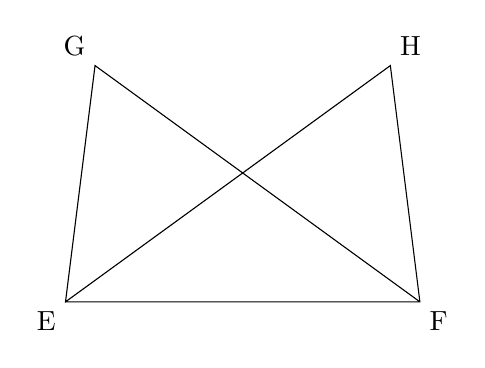
\begin{tikzpicture}[scale=1.5]
    \coordinate[label=below left:E](E)at(0,0);
    \coordinate[label=below right:F](F)at(3,0);
    \coordinate[label=above right:H](H)at(2.75,2);
    \coordinate[label=above left:G](G)at(0.25,2);
    \draw(E)--(F)--(H)--(E)--(G)--(F);
\end{tikzpicture}\par}
\begin{enumerate}
    \item Coder la figure ci-dessus en utilisant les informations de l'énoncé.
    \item Démontrer que EH = FG.
\end{enumerate}
\end{document}
